\documentclass[a4,12pt]{scrartcl}

%Basic 
\usepackage[utf8]{inputenc}
\usepackage[ngerman]{babel}
\usepackage[T1]{fontenc}
%Schrift 
%\usepackage{fontspec} 
%\setmainfont{Arial} 
%Zeilenabstand
\usepackage{setspace}
\setstretch {1.3}
\usepackage{float}
\usepackage[bottom = 3.50cm]{geometry}

%Titel Seite
\usepackage{titling} %Wird benötigt damit \maketitle die Variabeln title, author und date nicht überschreibt
\title{Test Cases}
%\subtitle{Projekt: software name}
\author{David Meister \and Andreas Stalder}		
 %mit /and können Personen hinzugefügt werden
\date{\today}


%Kopf, Fusszeile
\usepackage{fancyhdr}
\pagestyle{fancy}
\lhead{}
\chead{}
\rhead{Architektur}
\lfoot{\thetitle \: v1.0 }
\cfoot{\today}
\rfoot{Seite \thepage}
\renewcommand{\headrulewidth}{0.4pt}

%Bilder
\usepackage{graphicx}

%Zeichnen
\usepackage{tikz}

%Tabellen
\usepackage{booktabs}
\usepackage{longtable}

%Codesnippets
\usepackage{listings}
\lstset{language=java,basicstyle=\footnotesize,frame=single} %backgroundcolor=\color{lightgray}

%Querformat für eine Seite
\usepackage{lscape}
\usepackage{rotating}
\usepackage{pdflscape}

%URL 
\usepackage[colorlinks=true, linkcolor=blue, urlcolor=blue, citecolor=blue]{hyperref}
\urlstyle{same} 


%Loremimpsum
\usepackage{lipsum}



\begin{document}

%\clearpage\maketitle
\begin{titlepage}
	\centering
	\vspace{5cm}
	\begin{center}
%	\includegraphics[width=0.50\textwidth]{}
	\end{center}
%	{\huge\bfseries software name\par}
	\vspace{8cm}
	\raggedright
	{\bfseries HSR Studienarbeit Network Unit Testing\par}
	{\huge\bfseries Architektur \par}
	\vspace{1cm}
	{\theauthor \par}
	{\today\par}

\end{titlepage}

\section{Änderungsgeschichte}

\begin{table}[htb]
\centering
    \begin{tabular}{@{} l l l l@{}}\toprule    
    {Datum} & {Version} & {Änderung} & {Autor}\\ \midrule
    1.11.16 & 1.0 & Erstellung erster Version & dm/as\\ \addlinespace
    \end{tabular}
\caption{\textbf{Änderungsgeschichte}}
\end{table}

\newpage

%\thispagestyle{empty}
\tableofcontents
\newpage


\section{Einführung}
\subsection{Zweck}
Todo Architektur Zweck
\subsection{Gültigkeitsbereich}
Dieses Dokument ist über die gesamte Projektdauer gültig. Es wird in späteren Iterationen angepasst. Somit ist jeweils die neuste Version des Dokuments gültig und alte Versionen sind obsolet.
\subsection{Referenzen}
\begin{description}
Todo Ref zu Automation Plattform und anderen Dokumenten
\end{description}
\newpage
\section{Systemübersicht}
\newpage
\section{Klassenstruktur}
\newpage
\section{Logische Architektur}
\begin{figure} [H]
	\begin{center}
	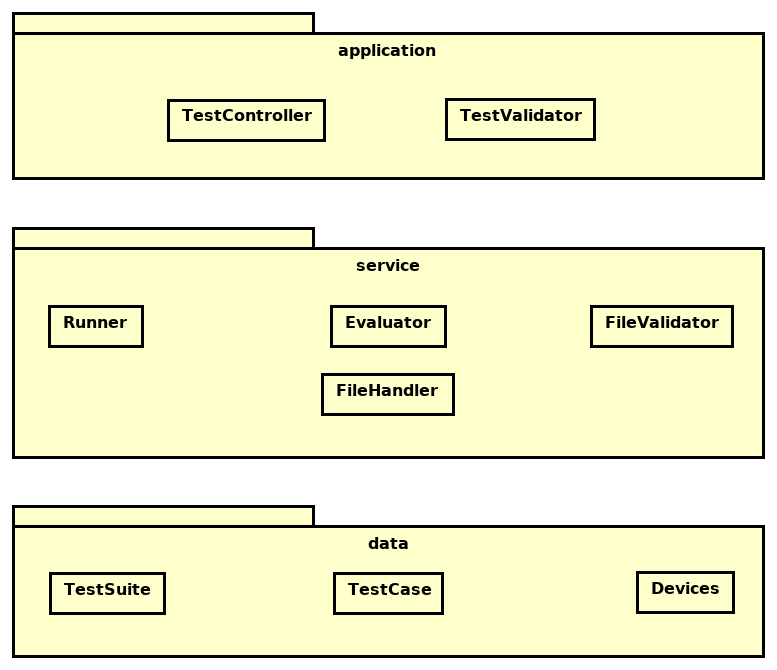
\includegraphics[width=0.90\textwidth]{./pictures/architektur.png}
	\label{Bild Referenz}
	\end{center}
\end{figure}
\begin{figure} [H]
	\begin{center}
	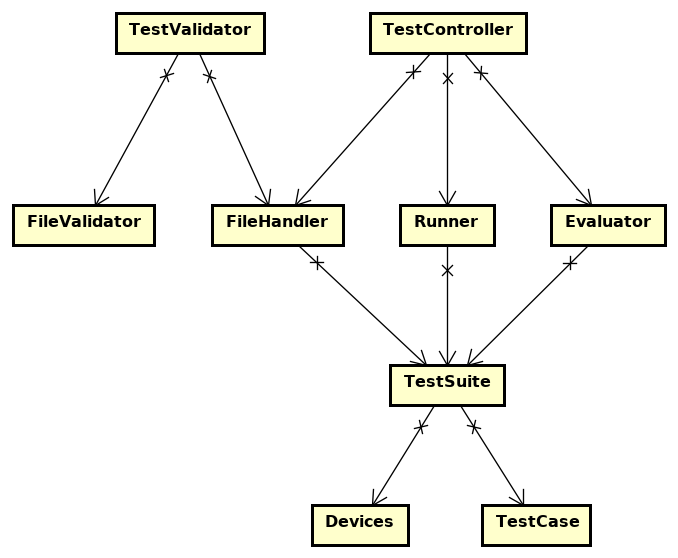
\includegraphics[width=0.90\textwidth]{./pictures/dependence_diagram.png}
	\label{Bild Referenz}
	\end{center}
\end{figure}


\subsection{Application-Layer}
wef
\subsubsection{Klassenstruktur}
\begin{table}[H]
\centering
    \begin{tabular}{@{}l p{11cm} @{}}\toprule    
    {Klassenname} & {Beschreibung}\\ \midrule
    ValidatorController & Der ValidatorController beinhaltet  \\       
    TestController & Das MainGUI ist die Hauptoberfläche. Von dieser aus wird alles gestartet und eingestellt. Diese Oberfläche führt auch zum InterfaceGUI. \\
    \bottomrule
    \end{tabular}
\end{table}
\subsubsection{Schnittstellen}
Der Presentation-Layer hat eine Schnittstelle zum Application-Layer, sowie zum Service-Layer. 
Das Mai hat eine Schnittstelle zum AudioPlayer, um diesen mittels GUI-Button zu starten und zu stoppen.
Zusätzlich besteht noch eine Schnittstelle zum SessionHandler, um die Session zu verwalten.
Eine weitere Schnittstelle besteht zum PacketScanner, damit dieser gesteuert werden kann.







\newpage
\section{Datensicherung}
Nuts speichert nur sehr wenige Daten. Dazu gehört ein Result-Log pro Ausführung und ein Error-Log für die Fehler.
\subsection{Testdateien}
Die erstellten Testdateien müssen von jedem Benutzer selber abgespeichert und verwaltet werden. Nuts speichert diese selber nicht ab.
\subsection{Auswertungen}
Jeder ausgeführte Test ergibt eine Log-Datei. Dieser Testlog wird unter /var/log/nuts/ gespeichert. Die Datei beinhaltet die Testergebnisse und weitere Details, falls der Test nicht bestanden ist.
\subsection{Error-Log}
Falls es beim ausführen des Programms zu einem Fehler kommt, wird dieser Fehler im Error-Log erfasst. Der Error-Log wird unter /var/log/nuts/error.log abgespeichert.

\end{document}

